\chapter{Introduction (Aufgabestellung)}
\label{chap:introduction}

In this work some experiments in formal verification of Scala code will be accomplished. 
The framework Stainless is used as a verification tool. The code of Bitcoin-S-Core, Scala implementation of Bitcoin, is taken as an input for Stainless to be verified. 
In following the main aspects of formal verification, Stainless and Bitcoin-S are described.

% Einträge im Verzeichnis erscheinen lassen ohne hier eine Referenz einzufügen
\nocite{kopka:band1}
\nocite{raichle:bibtex_programmierung}
\nocite{MiKTeX}
\nocite{KOMA}
\nocite{TeXnicCenter}
\nocite{Marti06}
\nocite{Erbsland08}
\nocite{juergens:einfuehrung}
\nocite{juergens:fortgeschritten}

\section{Formal verification (formal verification vs. simulation-based)}
\label{sec:formal_verification}

The longer and complexer a source code is, the more difficult it is to verify its correctness.
There are two main approaches for verification of program correctness. 

The commonly used one is the simulation-based verification.
To simulate a software design a set of some practical scenarios and assertions is created by a developer at the software testing stage. 
While testing it is tried to identify a design error by generating an input which can activate a bug.
It is not achievable to simulate all possible states and to test all possible inputs. 
Thus, a long-term test coverage model should be created to simulate a software design enough.
Furthermore it is challenging to test a software keeping the ability to observe the side effects of a specific part of code.
Practically, a developer runs tests, debugs appeared failures, adjustes a code of a software and extands a testbench verifying previously uncovered aspects. \cite{sanghavi:formal_verification}

Another powerfull method to discover whether a program works correct is formal verification. 
This is a systematic process based on mathematical modeling. 
It is unnecessary to create a simulation tests with some possible inputs. 
With formal verification all possible input values are explored algorithmically and exhaustively.
Correctness of a program is analyzed relative to its formal specification.
Formal specification is a mathematical description of a software behavior that can be provided to formal verification tools for proving it. \cite{sanghavi:formal_verification}

One of such tools is Stainless. It is used in this work to verify a Scala code.

 
%In figure \ref{fig:file_structure} the file structure is shown for this template.

%\begin{figure}[H]
%	\centering
%		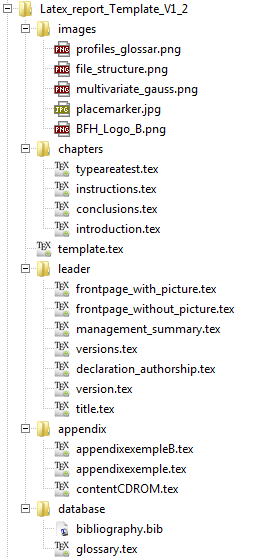
\includegraphics[scale=0.85]{images/file_structure.png}
%	\caption{File structure}
%	\label{fig:file_structure}
%\end{figure}

\section{Stainless (allgemeine Beschreibung: Struktur with pre- and postconditions, Solvers, Terminierung und mögliche Outputs)}
\label{sec:stainless}


Stainless is a framework developed by "Lab for Automated Reasoning and Analysis" (LARA) at EPFL's School of Computer and Communication Sciences to verify Scala programs.
It explores all input values, reports inputs for which a program fails and demonstrates counterexamples which violate a given specification.
The specification must be provided by a developer through giving a precondition and postcondition for functions. 

Constrains for input values are specified in a precondition with the keyword \textit{require}. 
Restrictions for received output values are defined in a postcondition with the keyword \textit{ensuring}. 
While compiling Stainless tries to prove that for the given input the postcondition of output always holds.
Three outcomes of the verification are possible: valid, unvalid and unknown when the framework is unable to prove or find a counterexample.
The code to be verified should be written in Pure Scala belonging to functional programming paradigm. To extend this subset of the Scala language Stainless supports also some imperative features translating them into Pure Scala concepts.
For more details about Stainless its official website can be explored. \cite{Stainless}

%\begin{table}[H]
%	\centering
%		\begin{tabular}{lll} \toprule
%			\textbf{First Name Last Name} & \textbf{E-mail} & \textbf{Function} \\ \midrule
%			Alfred Kaufmann & alfred.kaufmann@bfh.ch & Employer, Project Management, \\
%			& & Supplements, Improvements \\ \midrule
%			Fritz Dellsperger & Retired & Tips on the structure and layout \\ \midrule
%			David Burri & Contracted out & First compilation of the Template \\ \bottomrule
%		\end{tabular}
%	\caption{Contact Persons}
%	\label{tab:Contact Persons}
%\end{table}


\section{Bitcoin-S (Projekten und Packages, bitcoin-s-core, Eigenschaften zu prüfen)}
\label{sec:bitcoin_s}

%\begin{itemize}
%	\item Create a BFH Style Files
%	\item Template for the Compilation of presentations with \LaTeX{}
%\end{itemize}


